\section{Validación y Pruebas}

Se realizaron pruebas de funcionamiento con las mejores políticas para el brazo izquierdo y el brazo derecho siguiendo el protocolo presentado en la sección de Metodología previamente. \\

Como valores de umbral de precisión se tomaron los siguientes valores de distancia entre el efector final y la posición deseada, para la ejecución de las 1000 pruebas por cada agente:

\begin{itemize}
	\item 0.10 = 10 centímetros
	\item 0.075 = 7.5 centímetros
	\item 0.05 = 5 centímetros
\end{itemize}

\subsection{Evaluación de mejor política entrenada con PPO}

\subsubsection{Evaluación con agente brazo izquierdo}

La siguiente tabla resume los resultados de prueba para la ejecución de la política entrenada con \texttt{PPO-analytical-3} en el brazo izquierdo:

\begin{table}[h!]
	\centering
	\caption{Prueba para PPO sobre el brazo izquierdo}
	\label{tab:best-ppo-left}
	\begin{tabular}{|c|c|c|c|}
		\hline
		\textbf{Resultado} & \textbf{10cm} & \textbf{7.5cm} & \textbf{5cm} \\
		\hline
		Porcentaje de éxitos & 91.6\% & 81.1\% & 52.3\% \\
		\hline
		Error promedio (m) & 0.1103 & 0.1057 & 0.1303 \\
		\hline
		Desv. Estándar Error (m) & 0.0640 & 0.0914 & 0.1208 \\
		\hline
	\end{tabular}
\end{table}

\subsubsection{Evaluación con agente brazo derecho}

La siguiente tabla resume los resultados de prueba para la ejecución de la política entrenada con \texttt{PPO-analytical-3} en el brazo derecho:

\begin{table}[h!]
	\centering
	\caption{Prueba para PPO sobre el brazo derecho}
	\label{tab:best-ppo-right}
	\begin{tabular}{|c|c|c|c|}
		\hline
		\textbf{Resultado} & \textbf{10cm} & \textbf{7.5cm} & \textbf{5cm} \\
		\hline
		Porcentaje de éxitos & 92.1\% & 85.6\% & 66.0\% \\
		\hline
		Error promedio (m) & 0.1059 & 0.0930 & 0.1048 \\
		\hline
		Desv. Estándar Error (m) & 0.0619 & 0.0757 & 0.1091\\
		\hline
	\end{tabular}
\end{table}

\subsection{Evaluación de mejor política entrenada con SAC}

\subsubsection{Evaluación con agente brazo izquierdo}

La siguiente tabla resume los resultados de prueba para la ejecución de la política entrenada con \texttt{SAC-analytical-1} en el brazo izquierdo:

\begin{table}[h!]
	\centering
	\caption{Prueba para SAC sobre el brazo izquierdo}
	\label{tab:best-sac-left}
	\begin{tabular}{|c|c|c|c|}
		\hline
		\textbf{Resultado} & \textbf{10cm} & \textbf{7.5cm} & \textbf{5cm} \\
		\hline
		Porcentaje de éxitos & 97.2\% & 94.5\% & 69.2\% \\
		\hline
		Error promedio (m) & 0.0937 & 0.0739 & 0.0800 \\
		\hline
		Desv. Estándar Error (m) & 0.0162 & 0.0336 & 0.0740 \\
		\hline
	\end{tabular}
\end{table}

\subsubsection{Evaluación con agente brazo derecho}

La siguiente tabla resume los resultados de prueba para la ejecución de la política entrenada con \texttt{SAC-analytical-2} en el brazo derecho:

\begin{table}[h!]
	\centering
	\caption{Prueba para SAC sobre el brazo derecho}
	\label{tab:best-sac-right}
	\begin{tabular}{|c|c|c|c|}
		\hline
		\textbf{Resultado} & \textbf{10cm} & \textbf{7.5cm} & \textbf{5cm} \\
		\hline
		Porcentaje de éxitos & 94.3\% & 90.8\% & 72.8\% \\
		\hline
		Error promedio (m) & 0.0971 & 0.0782 & 0.0775 \\
		\hline
		Desv. Estándar Error (m) & 0.0352 & 0.0420 & 0.0740\\
		\hline
	\end{tabular}
\end{table}

\subsection{Comparación de éxito}

Teniendo en cuenta la cantidad de éxitos (sobre 1000 pruebas) para cada algoritmo, la siguiente gráfica permite visualizar una comparación de la efectividad de los algoritmos para entrenar políticas que permiten resolver el problema de la cinemática inversa en los brazos del robot Pepper con diferentes grados de precisión respecto a la ubicación final alcanzada respecto a la esperada.

\begin{figure}[h!]
	\centering
	
	\begin{subfigure}[b]{0.45\textwidth}
		\centering
		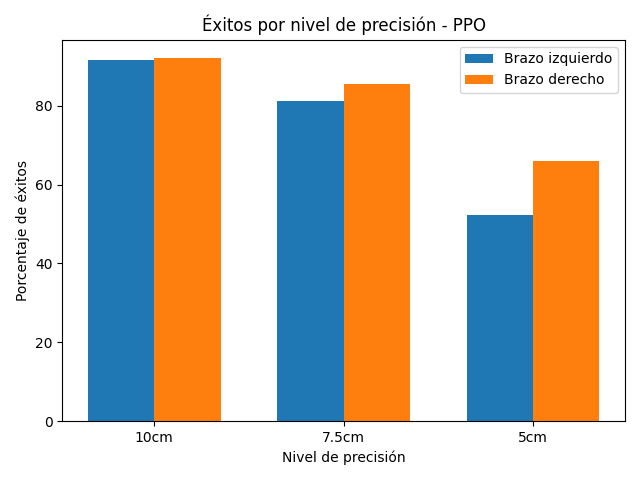
\includegraphics[width=\textwidth]{images/resultados/success_comparison_ppo}
		\caption{Éxitos de políticas entrenadas con PPO}
		\label{fig:ppo-test}
	\end{subfigure}
	\hfill
	\begin{subfigure}[b]{0.45\textwidth}
		\centering
		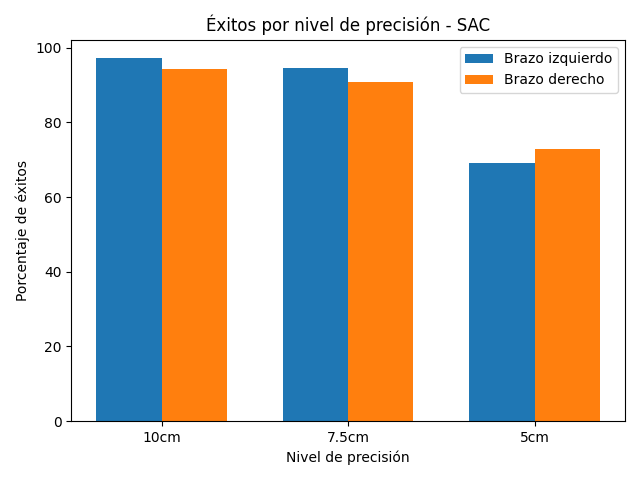
\includegraphics[width=\textwidth]{images/resultados/success_comparison_sac}
		\caption{Éxitos de políticas entrenadas con SAC}
		\label{fig:sac-test}
	\end{subfigure}
	
	\caption{Comparación de la cantidad de éxitos para diferentes umbrales de precisión}
	\label{fig:test-policy-success}
\end{figure}